\documentclass[12pt]{article}
%NOTE: This report format is 

\newcommand{\reporttitle}{Computer Project: Problem 5}
\newcommand{\reportauthorOne}{Tom BEAUVE}
\newcommand{\cidOne}{s224331}
\newcommand{\reportauthorTwo}{Benjamin BOCK}
\newcommand{\cidTwo}{S2304467}
\newcommand{\reportauthorThree}{Robby IRAKIZA}
\newcommand{\cidThree}{s224337}
\newcommand{\reportauthorFour}{Maxime LAYALLE}
\newcommand{\cidFour}{s195085}
\newcommand{\reportauthorFive}{Lilian STEIMETZ}
\newcommand{\cidFive}{s224403}
\newcommand{\reportauthorSix}{Hugo VANGEEBERGEN}
\newcommand{\cidSix}{s224178}
\newcommand{\reporttype}{Coursework}
\bibliographystyle{plain}

% include files that load packages and define macros
\usepackage{fontspec}
\usepackage{newtxtext,newtxmath} % Times New Roman pour texte et maths



% Packages utiles (ajoutez ceux dont vous avez besoin)
\usepackage[letterpaper,hmargin=2.8cm,vmargin=2.0cm,includeheadfoot]{geometry}
\usepackage{textpos}
\usepackage{natbib}
\usepackage{stackengine}
\usepackage{tabularx,longtable,multirow,subfigure,caption}%hangcaption
\usepackage{fncylab} %formatting of labels
\usepackage{fancyhdr}
\usepackage{color}
\usepackage[tight,ugly]{units}
\usepackage{url}
\usepackage{float}
\usepackage[english]{babel}
\usepackage{amsmath}
\usepackage{graphicx}
\usepackage[colorinlistoftodos]{todonotes}
\usepackage{dsfont}
\usepackage{epstopdf} % automatically replace .eps with .pdf in graphics
\usepackage{backref}
\usepackage{array}
\usepackage{etoolbox}
\usepackage{enumerate} % for numbering with [a)] format 
\usepackage{tcolorbox}
\usepackage{graphicx} % Pour insérer des images
\usepackage{tocloft}  % Pour personnaliser la liste des figures
\usepackage{hyperref}
% table of content
\renewcommand{\tableofcontentsname}{Table of Contents}

% equations numbering : (section.eqn number)
\numberwithin{equation}{section}
\renewcommand{\theequation}{\arabic{section}.\arabic{equation}}

% list enumeration
\usepackage{enumitem}

% table of figures
\renewcommand{\listfigurename}{Table of Figures}

% various theorems
\usepackage{ntheorem}
\theoremstyle{break}
\newtheorem{lemma}{Lemma}
\newtheorem{theorem}{Theorem}
\newtheorem{remark}{Remark}
\newtheorem{definition}{Definition}
\newtheorem{proof}{Proof}

% example-environment
\newenvironment{example}[1][]
{ 
\vspace{4mm}
\noindent\makebox[\linewidth]{\rule{\hsize}{1.5pt}}
\textbf{Example #1}\\
}
{ 
\noindent\newline\makebox[\linewidth]{\rule{\hsize}{1.0pt}}
}

\setlength{\parindent}{0em}  % indentation of paragraph

\setlength{\headheight}{14.5pt}
\pagestyle{fancy}
\fancyfoot[ER,OR]{\thepage}%Page no. in the left on
                                %odd pages and on right on even pages
\fancyfoot[OC,EC]{\sffamily }
\renewcommand{\headrulewidth}{0.1pt}
\renewcommand{\footrulewidth}{0.1pt}
\captionsetup{margin=10pt,font=small,labelfont=bf}

%--- chapter heading
\def\@makechapterhead#1{%
  \vspace*{10\p@}%
  {\parindent \z@ \raggedright
    \interlinepenalty\@M
    \Huge \bfseries 
    \thechapter \space\space #1\par\nobreak
    \vskip 30\p@
  }}

%---chapter heading for \chapter*  
\def\@makeschapterhead#1{%
  \vspace*{10\p@}%
  {\parindent \z@ \raggedright
    \interlinepenalty\@M
    \Huge \bfseries  
    #1\par\nobreak
    \vskip 30\p@
  }}

% %%%%%%%%%%%%% boxit
\def\Beginboxit
   {\par
    \vbox\bgroup
	   \hrule
	   \hbox\bgroup
		  \vrule \kern1.2pt %
		  \vbox\bgroup\kern1.2pt
   }

\def\Endboxit{%
			      \kern1.2pt
		       \egroup
		  \kern1.2pt\vrule
		\egroup
	   \hrule
	 \egroup
   }	

\newenvironment{boxit}{\Beginboxit}{\Endboxit}
\newenvironment{boxit*}{\Beginboxit\hbox to\hsize{}}{\Endboxit}

\allowdisplaybreaks

\makeatletter
\newcounter{elimination@steps}
\newcolumntype{R}[1]{>{\raggedleft\arraybackslash$}p{#1}<{$}}
\def\elimination@num@rights{}
\def\elimination@num@variables{}
\def\elimination@col@width{}
\newenvironment{elimination}[4][0]
{
    \setcounter{elimination@steps}{0}
    \def\elimination@num@rights{#1}
    \def\elimination@num@variables{#2}
    \def\elimination@col@width{#3}
    \renewcommand{\arraystretch}{#4}
    \start@align\@ne\st@rredtrue\m@ne
}
{
    \endalign
    \ignorespacesafterend
}
\newcommand{\eliminationstep}[2]
{
    \ifnum\value{elimination@steps}>0\leadsto\quad\fi
    \left[
        \ifnum\elimination@num@rights>0
            \begin{array}
            {@{}*{\elimination@num@variables}{R{\elimination@col@width}}
            |@{}*{\elimination@num@rights}{R{\elimination@col@width}}}
        \else
            \begin{array}
            {@{}*{\elimination@num@variables}{R{\elimination@col@width}}}
        \fi
            #1
        \end{array}
    \right]
    & 
    \begin{array}{l}
        #2
    \end{array}
    &%                                    moved second & here
    \addtocounter{elimination@steps}{1}
}
\makeatother

%% Fast macro for column vectors
\makeatletter  
\def\colvec#1{\expandafter\colvec@i#1,,,,,,,,,\@nil}
\def\colvec@i#1,#2,#3,#4,#5,#6,#7,#8,#9\@nil{% 
  \ifx$#2$ \begin{bmatrix}#1\end{bmatrix} \else
    \ifx$#3$ \begin{bmatrix}#1\\#2\end{bmatrix} \else
      \ifx$#4$ \begin{bmatrix}#1\\#2\\#3\end{bmatrix}\else
        \ifx$#5$ \begin{bmatrix}#1\\#2\\#3\\#4\end{bmatrix}\else
          \ifx$#6$ \begin{bmatrix}#1\\#2\\#3\\#4\\#5\end{bmatrix}\else
            \ifx$#7$ \begin{bmatrix}#1\\#2\\#3\\#4\\#5\\#6\end{bmatrix}\else
              \ifx$#8$ \begin{bmatrix}#1\\#2\\#3\\#4\\#5\\#6\\#7\end{bmatrix}\else
                 \PackageError{Column Vector}{The vector you tried to write is too big, use bmatrix instead}{Try using the bmatrix environment}
              \fi
            \fi
          \fi
        \fi
      \fi
    \fi
  \fi 
}  
\makeatother

\robustify{\colvec} % various packages needed for maths etc.
% quick way of adding a figure
\newcommand{\fig}[3]{
 \begin{center}
 \scalebox{#3}{\includegraphics[#2]{#1}}
 \end{center}
}

%\newcommand*{\point}[1]{\vec{\mkern0mu#1}}
\newcommand{\ci}[0]{\perp\!\!\!\!\!\perp} % conditional independence
\newcommand{\point}[1]{{#1}} % points 
\renewcommand{\vec}[1]{{\boldsymbol{{#1}}}} % vector
\newcommand{\mat}[1]{{\boldsymbol{{#1}}}} % matrix
\newcommand{\R}[0]{\mathds{R}} % real numbers
\newcommand{\Z}[0]{\mathds{Z}} % integers
\newcommand{\N}[0]{\mathds{N}} % natural numbers
\newcommand{\nat}[0]{\mathds{N}} % natural numbers
\newcommand{\Q}[0]{\mathds{Q}} % rational numbers
\ifxetex
\newcommand{\C}[0]{\mathds{C}} % complex numbers
\else
\newcommand{\C}[0]{\mathds{C}} % complex numbers
\fi
\newcommand{\tr}[0]{\text{tr}} % trace
\renewcommand{\d}[0]{\mathrm{d}} % total derivative
\newcommand{\inv}{^{-1}} % inverse
\newcommand{\id}{\mathrm{id}} % identity mapping
\renewcommand{\dim}{\mathrm{dim}} % dimension
\newcommand{\rank}[0]{\mathrm{rk}} % rank
\newcommand{\determ}[1]{\mathrm{det}(#1)} % determinant
\newcommand{\scp}[2]{\langle #1 , #2 \rangle}
\newcommand{\kernel}[0]{\mathrm{ker}} % kernel/nullspace
\newcommand{\img}[0]{\mathrm{Im}} % image
\newcommand{\idx}[1]{{(#1)}}
\DeclareMathOperator*{\diag}{diag}
\newcommand{\E}{\mathds{E}} % expectation
\newcommand{\var}{\mathds{V}} % variance
\newcommand{\gauss}[2]{\mathcal{N}\big(#1,\,#2\big)} % gaussian distribution N(.,.)
\newcommand{\gaussx}[3]{\mathcal{N}\big(#1\,|\,#2,\,#3\big)} % gaussian distribution N(.|.,.)
\newcommand{\gaussBig}[2]{\mathcal{N}\left(#1,\,#2\right)} % see above, but with brackets that adjust to the height of the arguments
\newcommand{\gaussxBig}[3]{\mathcal{N}\left(#1\,|\,#2,\,#3\right)} % see above, but with brackets that adjust to the height of the arguments
\DeclareMathOperator{\cov}{Cov} % covariance (matrix) 
\ifxetex
\renewcommand{\T}[0]{^\top} % transpose
\else
\newcommand{\T}[0]{^\top}
\fi
% matrix determinant
\newcommand{\matdet}[1]{
\left|
\begin{matrix}
#1
\end{matrix}
\right|
}



%%% various color definitions
\definecolor{darkgreen}{rgb}{0,0.6,0}

\newcommand{\blue}[1]{{\color{blue}#1}}
\newcommand{\red}[1]{{\color{red}#1}}
\newcommand{\green}[1]{{\color{darkgreen}#1}}
\newcommand{\orange}[1]{{\color{orange}#1}}
\newcommand{\magenta}[1]{{\color{magenta}#1}}
\newcommand{\cyan}[1]{{\color{cyan}#1}}


% redefine emph
\renewcommand{\emph}[1]{\blue{\bf{#1}}}

% place a colored box around a character
\gdef\colchar#1#2{%
  \tikz[baseline]{%
  \node[anchor=base,inner sep=2pt,outer sep=0pt,fill = #2!20] {#1};
    }%
}%
 % short-hand notation and macros


%%%%%%%%%%%%%%%%%%%%%%%%%%%%

\begin{document}
% front page
% Last modification: 2016-09-29 (Marc Deisenroth)
% Modification for UW: 2017-05-22 (jphickey)
\begin{titlepage}

\newcommand{\HRule}{\rule{\linewidth}{0.5mm}} % Defines a new command for the horizontal lines, change thickness here


%----------------------------------------------------------------------------------------
%	LOGO SECTION
%----------------------------------------------------------------------------------------



\begin{center} % Center remainder of the page

%----------------------------------------------------------------------------------------
%	HEADING SECTIONS
%----------------------------------------------------------------------------------------


\includegraphics[width = 15cm]{./figures/uliege_faculte_sciencesappliquees_logo_rvb}\\[1.5cm] 
\textbf{\textsc{\Large MECA0036-2 Finite Element Method}}\\[1.0cm] 
\textsc{\Large University of Liège}\\[0.5cm] 
\textsc{\large Faculty of Applied Sciences}\\[0.95cm] 

%----------------------------------------------------------------------------------------
%	TITLE SECTION
%----------------------------------------------------------------------------------------

\HRule \\[0.4cm]
{ \huge \bfseries \reporttitle}\\ % Title of your document
\HRule \\[1.5cm]
\end{center}
%----------------------------------------------------------------------------------------
%	AUTHOR SECTION
%----------------------------------------------------------------------------------------

%\begin{minipage}{0.4\hsize}

\begin{center}
    \begin{minipage}{0.45\linewidth} % Bloc à gauche
        \raggedright % Aligné à gauche
        \normalsize \textit{Professor:} \\
            \small Jean-Philippe PONTHOT
    \end{minipage}
    \begin{minipage}{0.45\linewidth} % Bloc à droite
        \raggedleft % Aligné à droite
        \normalsize \textit{Authors:} \\
        \begin{small}
            \reportauthorOne~(\cidOne)\\
            \reportauthorTwo~(\cidTwo)\\
            \reportauthorThree~(\cidThree)\\
            \reportauthorFour~(\cidFour)\\
            \reportauthorFive~(\cidFive)\\
            \reportauthorSix~(\cidSix)\\
        \end{small}
    \end{minipage}
\end{center}


\vspace{4cm}
\makeatletter
Date: \@date 

\vfill % Fill the rest of the page with whitespace



\makeatother

\end{titlepage}




%%%%%%%%%%%%%%%%%%%%%%%%%%% table of content
%If a table of content is needed, simply uncomment the following lines
\renewcommand{\contentsname}{Table of Content}

\tableofcontents
\newpage
\listoffigures
\newpage
\listoftables
\newpage

%%%%%%%%%%%%%%%%%%%%%%%%%%%% Main document
\section{Introduction}



\section{Strength of Materials}



\begin{equation}
\underline{\mathbf{u}} =
\begin{pmatrix}
    u(x,y,z) \\
    v(x,y,z) \\
    w(x,y,z)
\end{pmatrix}, \quad
\underline{\underline{\boldsymbol{\sigma}}} =
\begin{pmatrix}
    \sigma_{xx} & \sigma_{xy} & \sigma_{xz} \\
    \sigma_{yx} & \sigma_{yy} & \sigma_{yz} \\
    \sigma_{zx} & \sigma_{zy} & \sigma_{zz}
\end{pmatrix}, \quad
\underline{\underline{\boldsymbol{\varepsilon}}} =
\begin{pmatrix}
    \varepsilon_{xx} & \varepsilon_{xy} & \varepsilon_{xz} \\
    \varepsilon_{yx} & \varepsilon_{yy} & \varepsilon_{yz} \\
    \varepsilon_{zx} & \varepsilon_{zy} & \varepsilon_{zz}
\end{pmatrix}
\end{equation}

\subsection{Hypotheses for the general equations} \label{sec: SoM general hyp}
\begin{itemize}
    \item Linear Elastic material
    \item Isotropic material
    \item Continuous Medium
\end{itemize}

\subsection{General Equations}

\subsubsection{Equilibrium Equations}
\paragraph{Volume Equilibrium}
\begin{equation}
    \frac{\partial\sigma_{ij}}{\partial x_j} + F_i = 0
    \label{eqn: SoM volume equilibrium}
\end{equation}
\paragraph{Surface equilibrium}
\begin{equation}
    T_j = n_i \sigma_{ij}
    \label{eqn: SoM surface equilibrium}
\end{equation}
\paragraph{Moment equilibrium}
\begin{equation}
    \sigma_{ij} = \sigma_{ji}
\end{equation}

\subsubsection{Displacement-Strain Relation}
Compatibility Equation
\begin{equation}
    \underline{\underline{\boldsymbol{\varepsilon}}} = \frac{1}{2} ( \nabla \underline{u} + (\nabla \underline{u})^T )  
    \quad ; \quad  
    \varepsilon_{ij} = \frac{1}{2} \left( \frac{\partial u_i}{\partial x_j} + \frac{\partial u_j}{\partial x_i} \right)
    \label{eqn: SoM displacement-stress }
\end{equation}
We note that the strain tensor is symmetric, as $\varepsilon_{ij} = \varepsilon_{ji}$\\

Saint venant ( optional ? ), that the strain field has to respect
\begin{equation}
    D_{kk} \, \varepsilon_{ij} + D_{ij} \, \varepsilon_{kk} - D_{jk} \, \varepsilon_{ik} - D_{ik} \, \varepsilon_{jk} = 0
\end{equation}

\noindent where 
\begin{equation}
    D_{ij} = \frac{\partial^2}{\partial x_i \partial x_j}
\end{equation}


\subsubsection{Stress-Strain Relation}
Hooke's law : Elastic Linear 
\begin{equation}
    \underline{\underline{\boldsymbol{\sigma}}} = \underline{\underline{\underline{\underline{\boldsymbol{H}}}}} \space \underline{\underline{\boldsymbol{\varepsilon}}}
    \quad ; \quad 
    \sigma_{ij} = H_{ijkl} \space \varepsilon_{kl}
    \label{eqn: SoM stress-strain}
\end{equation}
Using : symmetric stress and strain tensors and isotropic material assumption, we can get 
\begin{equation}
    \begin{pmatrix}
    \varepsilon_{11} \\
    \varepsilon_{22} \\
    \varepsilon_{33} \\
    \gamma_{12} \\
    \gamma_{23} \\
    \gamma_{13}
    \end{pmatrix}= \frac{1}{E}\begin{pmatrix}
    1 & - \nu & -\nu & 0 & 0 & 0 \\
    -\nu & 1 & -\nu & 0 & 0 & 0 \\
    -\nu & -\nu & 1 & 0 & 0 & 0 \\
     &  &  & 2(1+\nu) & 0 & 0 \\
     &  \text{SYM}&  &  & 2(1+\nu) & 0 \\
     &  &  &  &  & 2(1+\nu)
    \end{pmatrix}
    \begin{pmatrix}
    \varepsilon_{11} \\
    \varepsilon_{22} \\
    \varepsilon_{33} \\
    \sigma_{12} \\
    \sigma_{23} \\
    \sigma_{13}
    \end{pmatrix}
    \label{eqn: SoM simplified strain-stress, matrix form}
\end{equation}

\begin{equation}
    \begin{pmatrix}
    \sigma_{11} \\
    \sigma_{22} \\
    \sigma_{33} \\
    \sigma_{12} \\
    \sigma_{23} \\
    \sigma_{13}
    \end{pmatrix}= \frac{E}{(1+\nu)(1-2\nu)}\begin{pmatrix}
    (1-\nu) &  \nu & \nu & 0 & 0 & 0 \\
    \nu & (1-\nu) & \nu & 0 & 0 & 0 \\
    \nu & \nu & (1-\nu) & 0 & 0 & 0 \\
     &  &  & \frac{1-2\nu }{2} & 0 & 0 \\
     &  \text{SYM}&  &  & \frac{1-2\nu }{2} & 0 \\
     &  &  &  &  & \frac{1-2\nu }{2}
    \end{pmatrix}
    \begin{pmatrix}
    \varepsilon_{11} \\
    \varepsilon_{22} \\
    \varepsilon_{33} \\
    \gamma_{12} \\
    \gamma_{23} \\
    \gamma_{13}
    \end{pmatrix}
    \label{eqn: SoM simplified stress-strain, matrix form}
\end{equation}

with $\gamma_{ij} = 2 \, \varepsilon_{ij}$, expressed in [rad], which we can thus rewrite as 

\begin{equation}
    \varepsilon_{ij} = \frac{1}{E} \left[ (1+\nu) \sigma_{ij} - \nu \, \sigma_{\ell \ell} \, \delta_{ij} \right]
    \label{eqn: SoM simplified strain-stress, index form}
\end{equation}

\begin{equation}
    \sigma_{ij} = \frac{E}{(1+\nu)(1-2\nu)} \left[ (1 - 2\nu) \varepsilon_{ij} + \nu \, \varepsilon_{\ell \ell} \, \delta_{ij} \right]
    \label{eqn: SoM simplified stress-strain, index form}
\end{equation}

\subsubsection{Equilibrium equation using displacements \underline{\textbf{u}}}

Navier Equation :
\begin{comment}
 \begin{equation}
    \frac{E}{2(1+\nu)} \left( \frac{\partial^2u_i}{ \partial x_{j} ^2} + \frac{1}{1-2\nu} \, \frac{\partial^2u_i}{\partial x_i \partial x_j} \right) + F_i = 0
\end{equation}   
\end{comment}

\begin{equation}
    \frac{E}{2(1+\nu)} \left( D_{jj} \, u_i + \frac{1}{1-2\nu} D_{ij} \, u_i \right) + F_i = 0
\end{equation}

\subsubsection{Boundary conditions}

\begin{equation}
    \begin{pmatrix}
    u \\
    v \\
    w
    \end{pmatrix} 
    = 
    \begin{pmatrix}
    u_0 \\
    v_0 \\
    w_0
    \end{pmatrix}
\end{equation}
on $\Gamma_u$, the clamped surface, where displacements are imposed.

\begin{equation}
    T_j = n_i \sigma_{ij}
\end{equation}
with $q$ and $\mu q$ on $\Gamma_q$, where forces are applied.

\begin{equation}
    \begin{pmatrix}
    u \\
    v \\
    w
    \end{pmatrix} 
    = 
    \begin{pmatrix}
    u_0 \\
    v_0 \\
    w_0
    \end{pmatrix}
    \quad \text{on } \Gamma_u, \text{ the clamped surface, where displacements are imposed.}
\end{equation}

\begin{equation}
    T_j = n_i \sigma_{ij} \quad \text{with } T_j \text{ = q or $\mu$q on } \Gamma_q, \text{ where forces are applied. }
\end{equation}


\subsection{Simplifying hypotheses}
In addition to the general hypotheses in subsection \ref{sec: SoM general hyp}, in order to study this problem analytically to get a first approximation of the solution, we add the following hypotheses : 
\begin{itemize}[itemsep = 1pt]
    \item Plane stress state ( applies for the entire problem)
    \item No body forces ( e.g. gravity)
    \item Linear elastic domain ( applies for the entire problem, we are searching $q_{max}$ such that we remain in the elastic domain)
    \item The ellipse at the bottom of the piece is replaced by an equivalent circle ( see details below)
    \item Stress concentration factors at fillet ( \textbf{congé de raccordement => anglais ?}), direction changes,... are neglected 
    \item Conservative Loading
\end{itemize}

As said above, the bottom elliptic ring is replaced by an equivalent cylinder. We do so by keeping the same area, so the equivalent radius is $\R_{eq} = \sqrt{a\, b}$ where $a$ and $b$ are the semi-axes of the ellipses. We thus obtain the equivalent cylinder represented in \autoref{fig: SoM ellipse approx}

\begin{figure}[H]
    \centering
    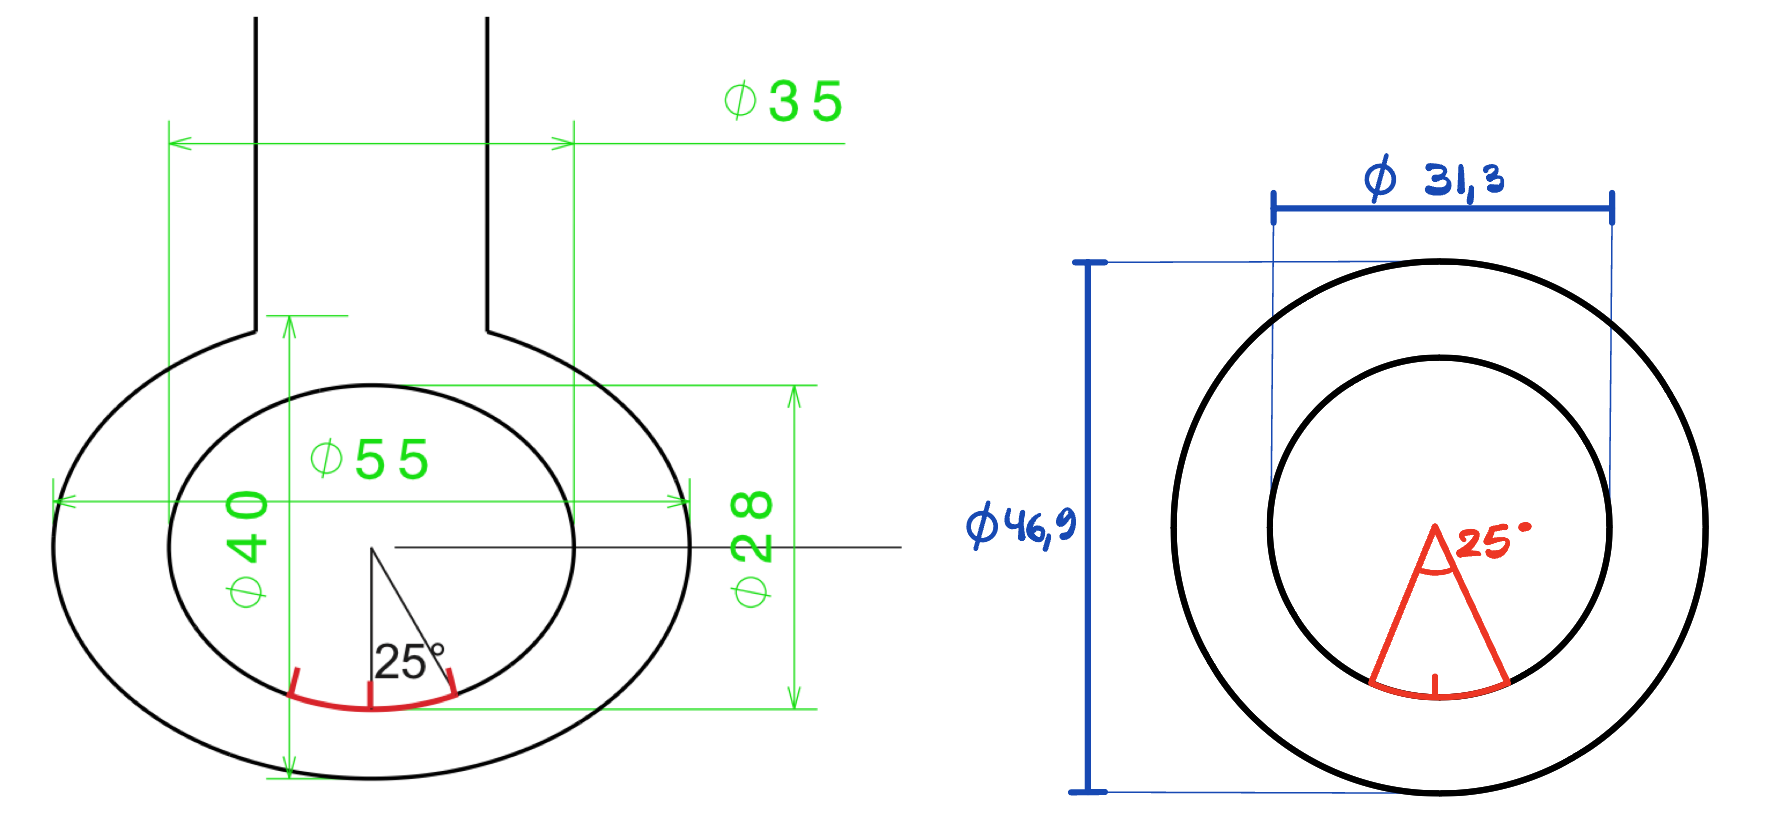
\includegraphics[width=0.7\textwidth]{Report/figures/SoM_ellipse_approx.png} 
    \caption{Appoximation used for the bottom ellipse}
    \label{fig: SoM ellipse approx}
\end{figure}

\subsection{Simplified Analysis}
Using the plane stress state, we can rewrite the stress tensor and the Hooke's law as 
\begin{equation}
    \underline{\underline{\boldsymbol{\sigma}}} =
\begin{pmatrix}
    \sigma_{xx} & \sigma_{xy} & 0 \\
    \sigma_{yx} & \sigma_{yy} & 0 \\
    0 & 0 & 0
\end{pmatrix}, \quad
\underline{\underline{\boldsymbol{\varepsilon}}} =
\begin{pmatrix}
    \varepsilon_{xx} & \varepsilon_{xy} & 0 \\
    \varepsilon_{yx} & \varepsilon_{yy} & 0\\
    0 & 0 & 0
\end{pmatrix}
\end{equation}
and, in polar coordinates, for the 2 cylinders 
\begin{equation}
    \underline{\underline{\boldsymbol{\sigma}}} =
    \begin{pmatrix}
        \sigma_{rr} & \sigma_{r\theta} & 0 \\
        \sigma_{\theta r} & \sigma_{\theta\theta} & 0 \\
        0 & 0 & \sigma_{zz}
    \end{pmatrix}, \quad
    \underline{\underline{\boldsymbol{\varepsilon}}} =
    \begin{pmatrix}
        \varepsilon_{rr} & \varepsilon_{r\theta} & 0 \\
        \varepsilon_{\theta r} & \varepsilon_{\theta\theta} & 0 \\
        0 & 0 & \varepsilon_{zz}
    \end{pmatrix}
\end{equation}
And equation ... rewrite as 

\begin{equation}
    \begin{pmatrix}
        \varepsilon_{11} \\
        \varepsilon_{22} \\
        \gamma_{12}
    \end{pmatrix}
    =
    \frac{1}{E}
    \begin{pmatrix}
        1 & -\nu & 0 \\
        -\nu & 1 & 0 \\
        0 & 0 & 2(1+\nu)
    \end{pmatrix}
    \begin{pmatrix}
        \sigma_{11} \\
        \sigma_{22} \\
        \sigma_{12}
    \end{pmatrix}
\end{equation}


\begin{equation}
    \begin{pmatrix}
    \sigma_{11} \\
    \sigma_{22} \\
    \sigma_{12} \\
    \end{pmatrix}= \frac{E}{(1-\nu^2)}\begin{pmatrix}
    1 &  \nu & 0  \\
    \nu & 1 & 0 \\
    0 & 0 & \frac{1-\nu}{2} 
    \end{pmatrix}
    \begin{pmatrix}
    \varepsilon_{11} \\
    \varepsilon_{22} \\
    \gamma_{12}
    \end{pmatrix}
\end{equation}


\subsubsection{Support Reactions in Cartesian Coordinates}

We consider the total resultant force $\mathbf{F}$ coming from the distributed loads applied on the upper arcs of the structure. These loads are decomposed into radial and tangential components, and then projected onto the Cartesian base vectors $\mathbf{e}_x$ and $\mathbf{e}_y$.

\begin{equation}
\boxed{
\mathbf{F} =
\int_{\Gamma_{q1}} (-q\, \mathbf{e}_r - \mu q\, \mathbf{e}_\theta) \, ds
+
\int_{\Gamma_{q2}} (q\, \mathbf{e}_r - \mu q\, \mathbf{e}_\theta) \, ds
}
\end{equation}

To project the radial and tangential vectors onto the Cartesian base:

\begin{align*}
\mathbf{e}_r \cdot \mathbf{e}_x &= \sin\theta, &
\mathbf{e}_r \cdot \mathbf{e}_y &= -\cos\theta \\
\mathbf{e}_\theta \cdot \mathbf{e}_x &= \cos\theta, &
\mathbf{e}_\theta \cdot \mathbf{e}_y &= \sin\theta
\end{align*}

\paragraph{Horizontal component \( F_x \):}
\begin{align}
F_x &=
\int_{\theta_{t1}^-}^{\theta_{t1}^+} (-q \sin\theta - \mu q \cos\theta) \, R_{\text{t,ext}} \, d\theta
+
\int_{\theta_{t2}^-}^{\theta_{t2}^+} (q \sin\theta - \mu q \cos\theta) \, R_{\text{t,int}} \, d\theta
\tag{2.25}
\end{align}

\begin{align*}
F_x &=
\int_{-60^\circ}^{-50^\circ} (-q \sin\theta - \mu q \cos\theta) \cdot 34 \, d\theta
+
\int_{50^\circ}^{60^\circ} (q \sin\theta - \mu q \cos\theta) \cdot 27.5 \, d\theta
\end{align*}

\begin{equation}
\begin{aligned}
F_x &= 34 \,q \Big[
    (\cos(-50^\circ) - \cos(-60^\circ) )
    - \mu \left( \sin(-50^\circ) - \sin(-60^\circ) \right)\Big] \\
&\qquad + 
27.5 \, q \Big[ 
    -(\cos(60^\circ) - \cos(50^\circ) )
    - \mu \left( \sin(60^\circ) - \sin(50^\circ) \right)
\Big] \\
&= \boxed{-0.6 \cdot q}
\end{aligned}
\tag{2.26}
\end{equation}

\paragraph{Vertical component \( F_y \):}
\begin{align}
F_y &=
\int_{\theta_{t1}^-}^{\theta_{t1}^+} (q \cos\theta - \mu q \sin\theta) \, R_{\text{ext}} \, d\theta
+
\int_{\theta_{t2}^-}^{\theta_{t2}^+} (-q \cos\theta - \mu q \sin\theta) \, R_{\text{int}} \, d\theta
\tag{2.27}
\end{align}

\begin{align*}
F_y &=
\int_{-60^\circ}^{-50^\circ} (q \cos\theta - \mu q \sin\theta) \cdot 68 \, d\theta
+
\int_{50^\circ}^{60^\circ} (-q \cos\theta - \mu q \sin\theta) \cdot 55 \, d\theta
\end{align*}

\begin{equation}
\begin{aligned}
F_y &= -q \Big[
68 \cdot \left( 
    \sin(-50^\circ) - \sin(-60^\circ)
    - \mu \left( \cos(-50^\circ) - \cos(-60^\circ) \right)
\right) \\
&\qquad + 
55 \cdot \left( 
    -\sin(60^\circ) + \sin(50^\circ)
    - \mu \left( \cos(60^\circ) - \cos(50^\circ) \right)
\right)
\Big] \\
&= \boxed{-0.93 \cdot q}
\end{aligned}
\tag{2.28}
\end{equation}

\subsubsection{Determination of support surface tensions with 50° contact angle}

In this section, we compute the surface tensions $\sigma_r$ and $\sigma_\theta$ at the internal support arc of the lower ring, assuming they are constant over the contact surface.

As previously determined, the total reaction force at the bottom must compensate the applied loads:
\[
\vec{F}_{\text{support}} = -\vec{F}_{\text{applied}} =
\begin{pmatrix}
+0.60 \cdot q \\
+0.93 \cdot q
\end{pmatrix}
\]

We now consider a more accurate angular contact range of $50^\circ$, symmetrically centered around the vertical axis:
\[
\theta_b^- = -25^\circ, \qquad \theta_b^+ = +25^\circ
\]

We model the surface stress field as:
\[
\vec{\sigma}(\theta) = \sigma_r \, \vec{e}_r + \sigma_\theta \, \vec{e}_\theta
\]

Projecting this field onto the Cartesian basis and integrating over the arc gives:

\begin{align*}
F_x &= R_{\text{int}} \int_{\theta_b^-}^{\theta_b^+} \left( \sigma_r \sin\theta + \sigma_\theta \cos\theta \right) d\theta \\
F_y &= R_{\text{int}} \int_{\theta_b^-}^{\theta_b^+} \left( -\sigma_r \cos\theta + \sigma_\theta \sin\theta \right) d\theta
\end{align*}

This can be written as a matrix system:
\[
R_{\text{int}} \cdot
\begin{pmatrix}
\int \sin\theta \, d\theta & \int \cos\theta \, d\theta \\
-\int \cos\theta \, d\theta & \int \sin\theta \, d\theta
\end{pmatrix}_{-25^\circ}^{25^\circ}
\begin{pmatrix}
\sigma_r \\
\sigma_\theta
\end{pmatrix}
=
\begin{pmatrix}
F_x \\
F_y
\end{pmatrix}
\]

Evaluating the integrals:
\[
\int_{-25^\circ}^{25^\circ} \sin\theta \, d\theta = \cos(-25^\circ) - \cos(25^\circ) = 0 \quad (\text{since cosine is even})
\]
\[
\int_{-25^\circ}^{25^\circ} \cos\theta \, d\theta = \sin(25^\circ) - \sin(-25^\circ) = 2 \cdot \sin(25^\circ) \approx 0.845

\Rightarrow
\text{Matrix} =
R_{\text{int}} \cdot
\begin{pmatrix}
0 & 0.845 \\
-0.845 & 0
\end{pmatrix}
\]

Substituting $R_{\text{int}} = 31.3$ mm and solving:

\[
\begin{pmatrix}
\sigma_r \\
\sigma_\theta
\end{pmatrix}
=
\frac{1}{31.3}
\cdot
\begin{pmatrix}
0 & -\frac{1}{0.845} \\
\frac{1}{0.845} & 0
\end{pmatrix}
\cdot
\begin{pmatrix}
0.60 \cdot q \\
0.93 \cdot q
\end{pmatrix}
\]

\[
\Rightarrow
\sigma_r = -\frac{0.93}{31.3 \cdot 0.845} \cdot q \approx \boxed{-0.0352 \cdot q} \quad [\text{MPa}]
\qquad
\sigma_\theta = \frac{0.60}{31.3 \cdot 0.845} \cdot q \approx \boxed{+0.0227 \cdot q} \quad [\text{MPa}]
\]

\subsubsection{Radial displacement analysis}

\paragraph{Axisymmetric simplification.} In order to obtain an analytical expression of the displacement field, we make a strong simplification by assuming that the problem is purely axisymmetric. This implies that:

\begin{itemize}
    \item All quantities depend only on the radial coordinate \( r \), not on the angular direction \( \theta \)
    \item There is no circumferential or axial displacement: \( u_\theta = u_z = 0 \)
    \item The displacement field is purely radial: \( \vec{u}(r, \theta) = u_r(r) \cdot \vec{e}_r \)
\end{itemize}

This is clearly an idealised assumption, especially since the actual geometry (e.g., contact arcs) is not perfectly axisymmetric. However, it allows us to reduce the problem to a 1D radial formulation and match it to a known analytical solution from the Mechanics of Solids course: a thick-walled cylinder under radial pressure.

\paragraph{Governing equation and general solution.} With this assumption and no body forces, the Navier equation in cylindrical coordinates becomes:

\[
\frac{d}{dr} \left( \frac{1}{r} \cdot \frac{d}{dr}(r u_r) \right) = 0
\]

Solving this equation yields the general form of the displacement:

\[
u_r(r) = A \cdot r + \frac{B}{r}
\]

\paragraph{Strains and stresses.} From this, we compute the radial and circumferential strains:

\[
\varepsilon_{rr} = \frac{du_r}{dr} = A - \frac{B}{r^2}, \qquad
\varepsilon_{\theta\theta} = \frac{u_r}{r} = A + \frac{B}{r^2}
\]

The identity \( \varepsilon_{\theta\theta} = \frac{u_r}{r} \) reflects the relative elongation of a circular arc of radius \( r \).

We then use the general tensorial form of Hooke’s law (Eq.~(2.12)):

\[
\sigma_{ij} = \frac{E}{(1 + \nu)(1 - 2\nu)} \left[ (1 - 2\nu)\varepsilon_{ij} + \nu \, \varepsilon_{\ell\ell} \, \delta_{ij} \right]
\]

Assuming \( \varepsilon_{zz} = 0 \), we find \( \varepsilon_{\ell\ell} = \varepsilon_{rr} + \varepsilon_{\theta\theta} = 2A \), and the radial stress becomes:

\[
\sigma_{rr}(r) = \frac{E}{(1 + \nu)(1 - 2\nu)} \left[ A + (\nu - 1) \cdot \frac{B}{r^2} \right]
\]
\paragraph{Top left (external contact).}

\textit{Boundary conditions:}
\[
\sigma_{rr}(R_1) = 0, \qquad \sigma_{rr}(R_2) = -q
\]

\textit{Constants obtained:}
\[
A = \frac{R_2^2 \cdot q \cdot (-2\nu^2 - \nu + 1)}{E (R_1^2 - R_2^2)}, \qquad
B = \frac{R_1^2 R_2^2 \cdot q \cdot (2\nu^2 + \nu - 1)}{E (R_1^2 (\nu - 1) + R_2^2 (1 - \nu))}
\]


\vspace{1em}

\paragraph{Top right (internal contact).}

\textit{Boundary conditions:}
\[
\sigma_{rr}(R_1) = q, \qquad \sigma_{rr}(R_2) = 0
\]

\textit{Constants obtained:}
\[
A = \frac{R_1^2 \cdot q \cdot (-2\nu^2 - \nu + 1)}{E (R_1^2 - R_2^2)}, \qquad
B = \frac{R_1^2 R_2^2 \cdot q \cdot (2\nu^2 + \nu - 1)}{E (R_1^2 (\nu - 1) + R_2^2 (1 - \nu))}
\]

\vspace{1em}

\paragraph{Bottom ring .}

\textit{Boundary conditions:}
\[
\sigma_{rr}(R_1) = \sigma_1, \qquad \sigma_{rr}(R_2) = 0
\]

\textit{Constants obtained:}
\[
A = \frac{R_1^2 \cdot \sigma_1 \cdot (-2\nu^2 - \nu + 1)}{E (R_1^2 - R_2^2)}, \qquad
B = \frac{R_1^2 R_2^2 \cdot \sigma_1 \cdot (2\nu^2 + \nu - 1)}{E (R_1^2 (\nu - 1) + R_2^2 (1 - \nu))}
\]


\newpage
\bibliography{mybib}


\end{document}
%%% Local Variables: 
%%% mode: latex
%%% TeX-master: t
%%% End: 
